\appendix
\section{Resoconto delle attività di verifica}
\subsection{Periodo di analisi e produzione del proof of concept}
In questa sezione sono raccolti i vari resoconti delle attività di verifica svolti nei periodi precedenti alla revisione RTB, ovvero il periodo di analisi e quello di produzione del proof of concept.
Dato che non sono ancora state svolte attività di progettazione e codifica del prodotto finale, verranno misurare solo le metriche riguardanti i processi attivi.
\subsubsection{Gestione processi}
\begin{figure}[H]
	\centering
	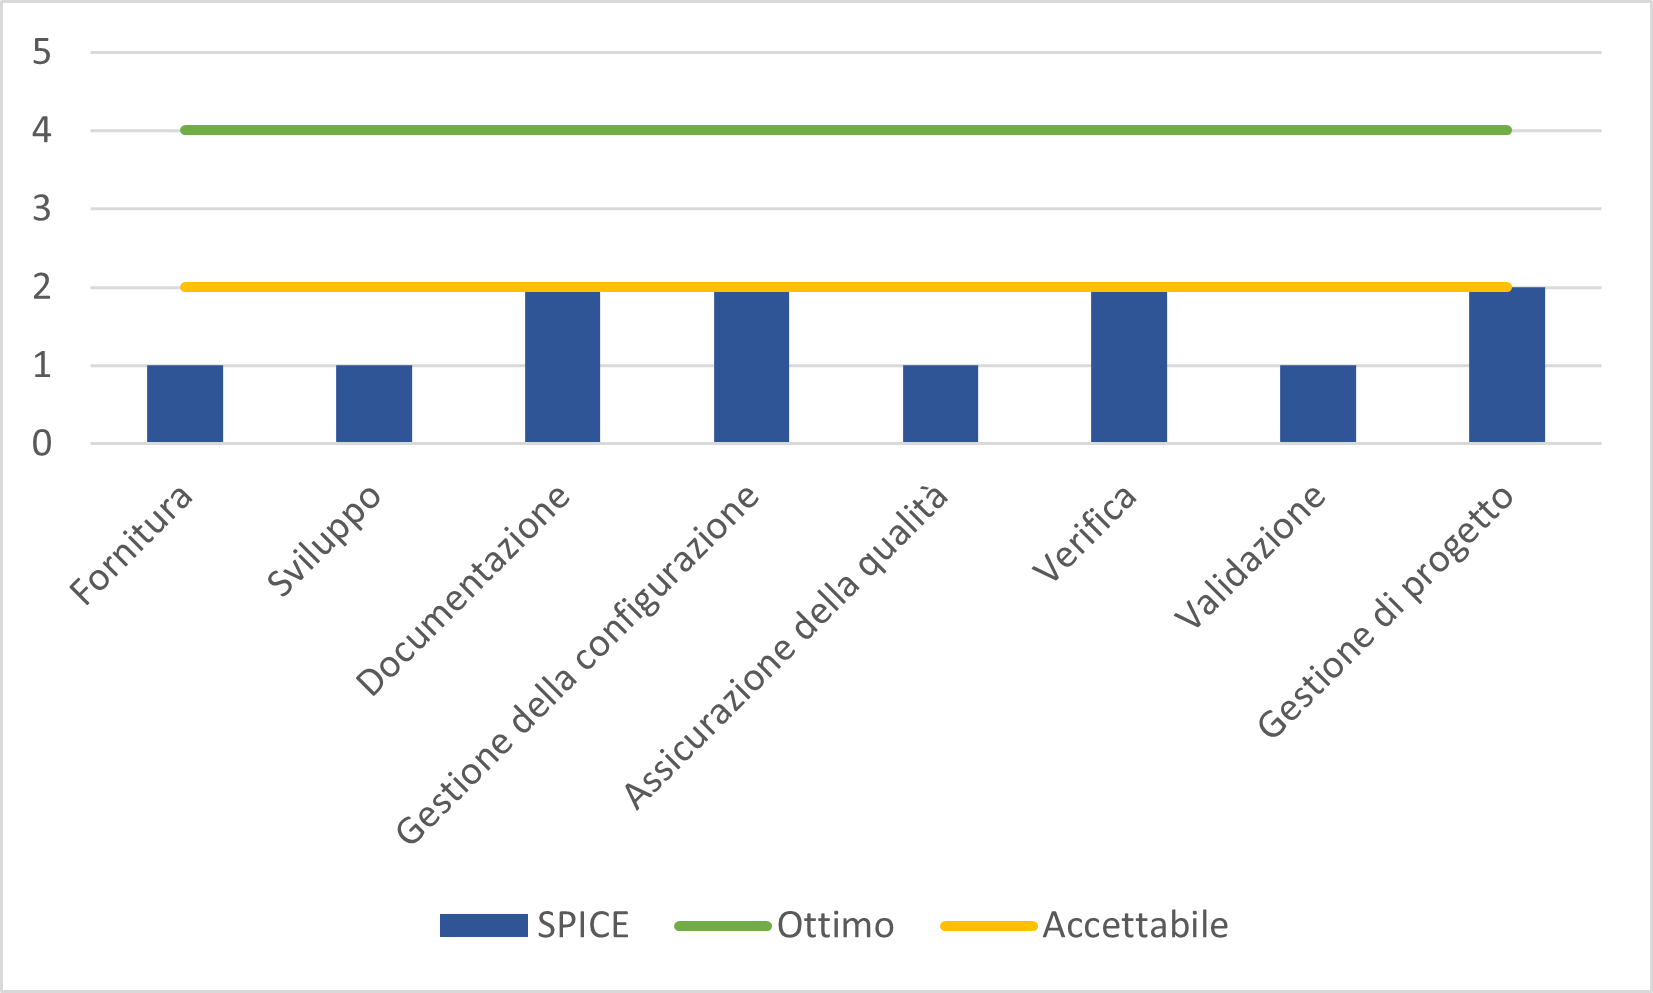
\includegraphics[scale=1.1]{img/SPICE.png}
	\caption{Livello di capacità dei processi attivi nel progetto}
\end{figure}
\paragraph{Analisi retrospettiva sui risultati}
\subsubsection{Pianificazione}
\subsubsubsection{Efficienza nell'utilizzo delle risorse}
\begin{figure}[H]
	\centering
	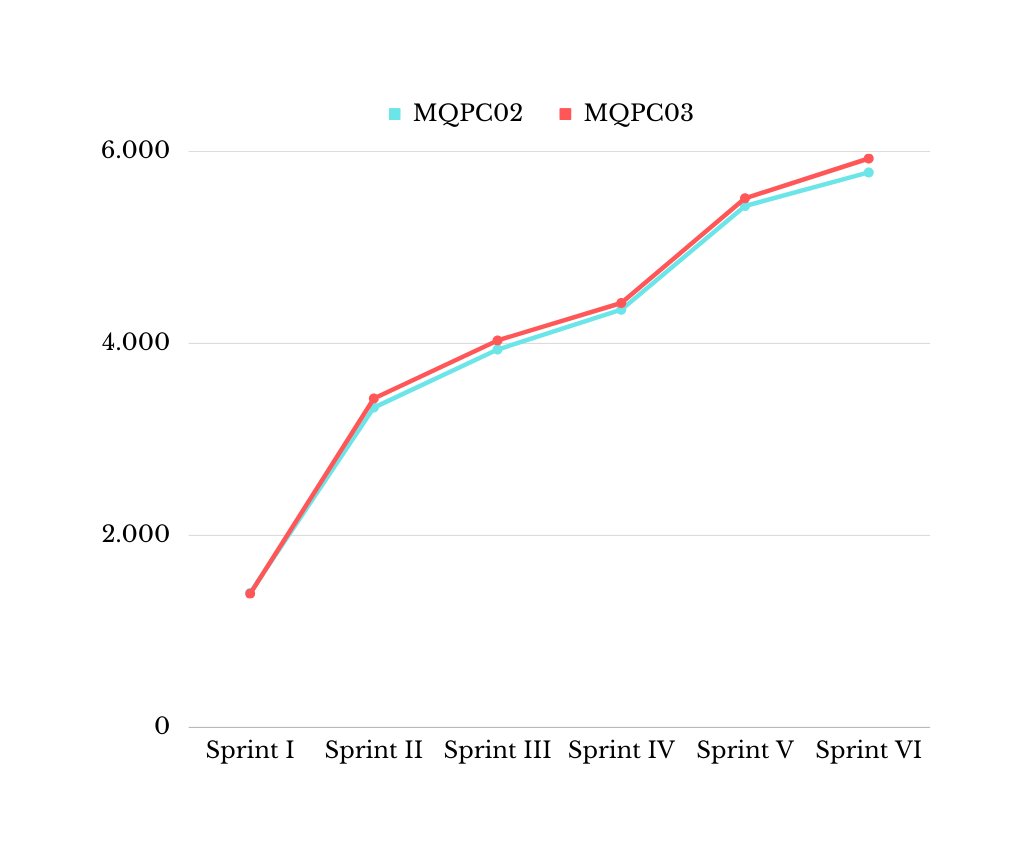
\includegraphics[scale=0.5]{img/BCWS-ACWS.png}
	\caption{Grafico che mostra l'andamento dei costi pianificati correlato a quelli reali}
\end{figure}
\paragraph{Analisi retrospettiva sui risultati}
\subsubsubsection{Variazioni dalla pianificazione}
\begin{figure}[H]
	\centering
	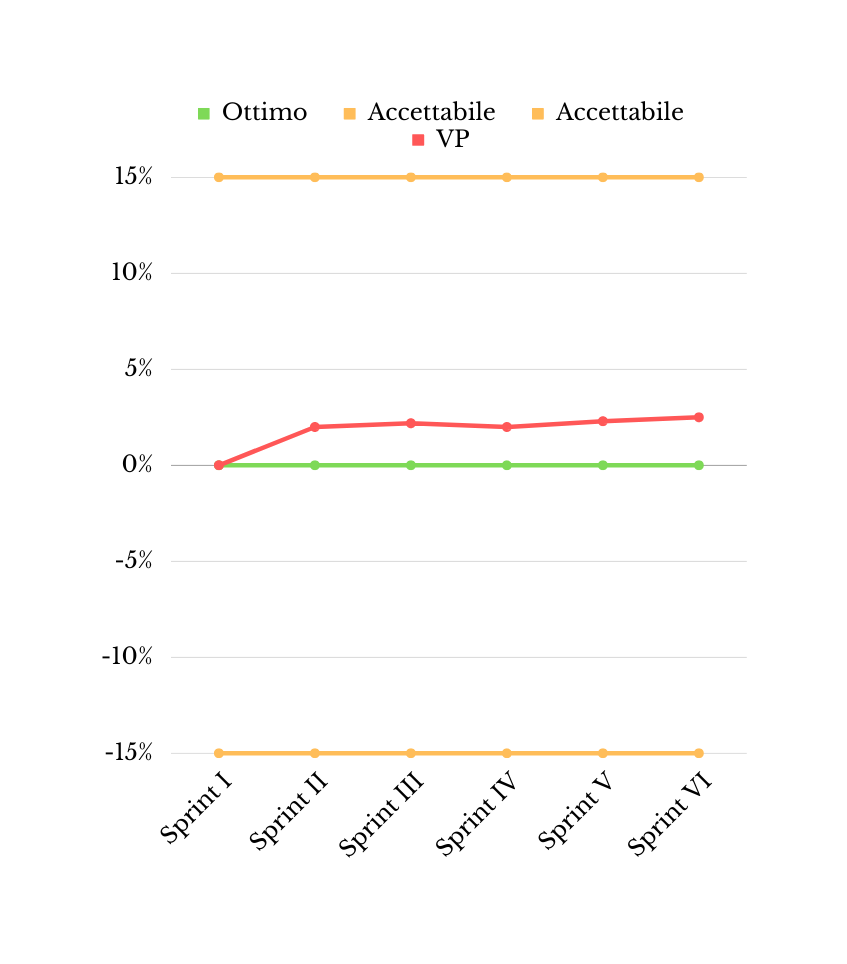
\includegraphics[scale=0.5]{img/SV.png}
	\caption{Grafico che mostra la differenza in percentuale tra le ore pianificate (ottime) e le ore effettivamente impiegate}
\end{figure}
\begin{figure}[H]
	\centering
	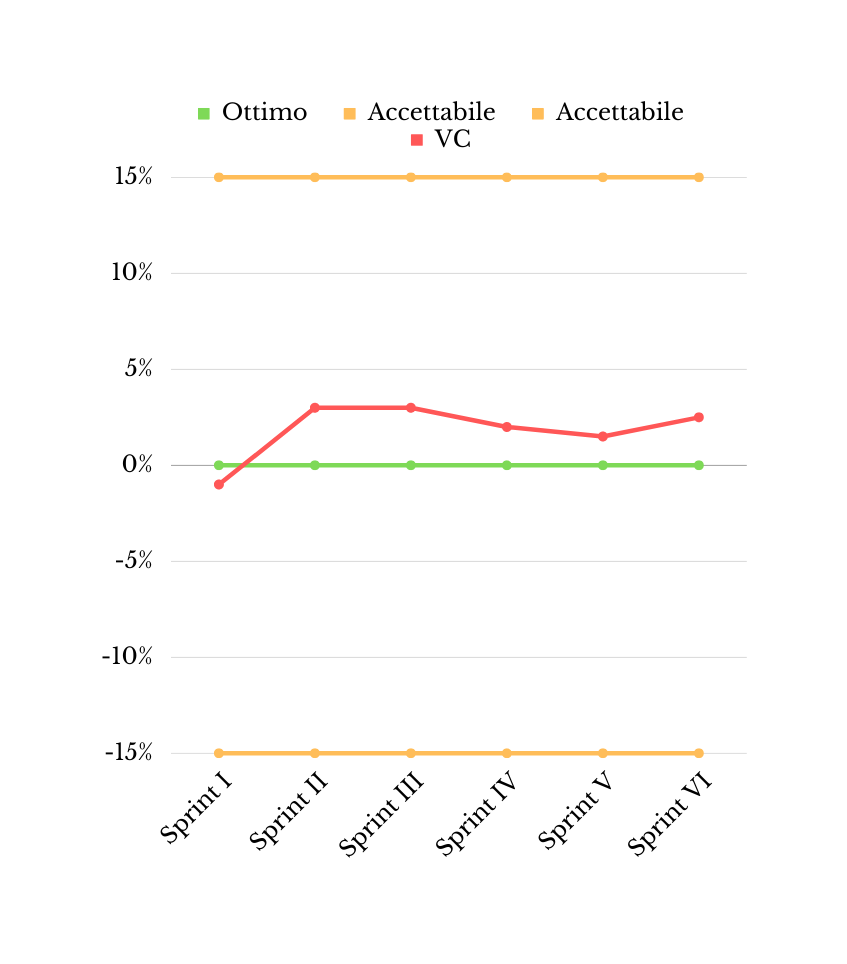
\includegraphics[scale=0.5]{img/CV.png}
	\caption{Grafico che mostra la differenza in percentuale tra i costi pianificati (ottimi) e i costi effettivi}
\end{figure}
\paragraph{Analisi retrospettiva sui risultati}
\subsubsection{Documentazione}
\subsubsubsection{Indice di Gulpease}
\begin{table}[H]
	\centering
	\setlength\extrarowheight{5pt}
	\rowcolors{2}{gray!10}{gray!40}
	\renewcommand\tabularxcolumn[1]{>{\Centering}m{#1}}
	\begin{tabularx}{\textwidth}{| c | X |} 
		\hline
		\rowcolor{white}
		\textbf{Documento} & \textbf{Valore}\\
		\hline
		\textit{Analisi\_dei\_Requisiti v 1.0.0} & 90 \\
		\hline
		\textit{Norme\_di\_Progetto v 1.0.0} & 75\\
		\hline
		\textit{Piano\_di\_Progetto v 1.0.0} & 68\\
		\hline
		\textit{Piano\_di\_Qualifica v 1.0.0} & 71\\
		\hline
		\textit{Glossario v 1.0.0} & 69\\
		\hline
		\rowcolor{white}
		\caption{Indice di Gulpease}
	\end{tabularx}
\end{table}
\paragraph{Analisi retrospettiva sui risultati}
I risultati ottenuti dai documenti sono soddisfacenti e superano la soglia che il gruppo ha definito accettabile. Tutti i documenti rilasciati hanno quindi un indice di leggibilità buono.
